\documentclass[a4paper,12pt,twoside,openright]{report}
%    \renewcommand{\baselinestretch}{1.6}      % interline spacing
%
% \includeonly{}
%
%			PREAMBOLO
%
\usepackage{amssymb,amsmath,amsthm}
\usepackage{graphicx}
\usepackage{url}
\usepackage{hyperref}
\usepackage{epsfig}
\usepackage[english]{babel}
\usepackage{setspace}
\usepackage{tesi}

\usepackage[
  a4paper,
  twoside,
  inner=3.5cm,
  outer=2.5cm,
  top=3cm,
  bottom=3cm,
  bindingoffset=0.5cm
]{geometry}

% per le accentate
\usepackage[utf8]{inputenc}
%
\newtheorem{myteor}{Teorema}[section]
%
\newenvironment{teor}{\begin{myteor}\sl}{\end{myteor}}

\renewcommand{\arraystretch}{1.5} % Padding verticale
%
%
%			TITOLO
%
\begin{document}
\title{REPRODUCTION AND ANALYSIS OF REAL-WORLD USE-AFTER-FREE ATTACKS AND STUDY OF DEFENCE TECHNIQUES}
\author{Stefano NAVA}
\dept{Corso di Laurea Magistrale in Informatica} 
\anno{2025-2026}
\matricola{123456}
\relatore{Prof. Andrea LANZI}
\correlatore{Dr. Andrea MONZANI}
%
%        \submitdate{month year in which submitted to GPO}
%		- date LaTeX'd if omitted
%	\copyrightyear{year degree conferred (next year if submitted in Dec.)}
%		- year LaTeX'd (or next year, in December) if omitted
%	\copyrighttrue or \copyrightfalse
%		- produce or don't produce a copyright page (false by default)
\figurespagetrue
%		- produce or don't produce a List of Figures page
%		  (false by default)
%	\tablespagetrue or \tablespagefalse
%		- produce or don't produce a List of Tables page
%		  (false by default)
% 
%			DEDICA
%
\beforepreface
%\prefacesection{}
%        {\hfill \Large {\sl dedicato a \dots}}
% 
%			PREFAZIONE
%
\prefacesection{Preface}

Software security is nowadays a fundamental aspect of the development and maintenance of IT systems. The increasing complexity of applications, combined with the growing interconnection between devices and services, has significantly expanded the attack surface that can be exploited by potential malicious actors. Operating systems, browsers, drivers and distributed services are critical components whose proper functioning is closely linked to the robustness of their security properties.

In this context, proper memory management plays a central role, particularly in systems developed using low-level languages such as C and C++, which are defined as non-memory-safe. Although these languages offer high performance and control over resources, they are particularly prone to memory management errors, which can result in exploitable vulnerabilities. Memory-safe languages, in fact, have automatic mechanisms for controlling the allocation and deallocation of memory blocks. In the absence of these, while memory access is faster, an important safeguard for security is lost.

Despite decades of research and the development of numerous mitigation techniques, such vulnerabilities continue to arise even in widely used and mature software, highlighting how memory security remains an ongoing challenge in the contemporary cybersecurity landscape.

%
%
%			ORGANIZZAZIONE - TODO
\section*{Organisation of the thesis}
\label{organizzazione}
The thesis is organised as follows:
\begin{itemize}
\item nel Capitolo 1 ....
\end{itemize}
%
%			RINGRAZIAMENTI
%
%\prefacesection{Ringraziamenti}
%asdjhgftry.

\afterpreface

\chapter{Background}

\section{Memory structure}
The memory, the primary target of an attack of this kind, has the following structure:

\begin{figure}[h]
    \centering
    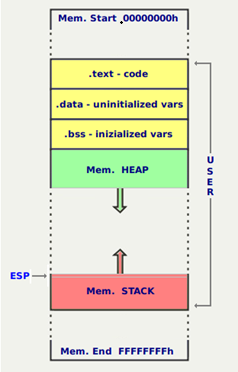
\includegraphics{images/stack-heap.png}
    \caption{Structure of memory areas.}
    \label{fig:stack_heap}
\end{figure}

\noindent The two areas primarily affected by attacks of this kind are the stack and the heap.

\subsection{Stack}
It is a data structure organised according to a LIFO (Last In, First Out) policy and used primarily for managing function calls. Each function call involves the creation of a stack frame, containing local variables, parameters and return information (such as the return address, which tells the program the point in the calling code from which to resume execution once the function has been exited). The allocation and deallocation of memory on the stack are automatic and handled by the compiler: when a function terminates, its corresponding frame is removed.

\subsection{Heap}
It is a memory region used for dynamic allocation, managed explicitly by the programr using primitives such as \texttt{malloc}/\texttt{free} in C or \texttt{new}/\texttt{delete} in C++. Unlike the stack, the heap does not follow a strict allocation order and allows for greater flexibility in managing the lifecycle of objects. However, it is precisely this flexibility that introduces complexity which can lead the programr into error.

\subsection{Pointers}\label{pointers}
In memory-unsafe languages, pointers are data structures that contain the address of a specific area of heap memory (to which they "point") and, for example in C, are initialised using the \texttt{malloc} function and freed using the \texttt{free} function. The programr can use them to perform operations both on the addresses they contain and on the values contained in the memory cells they point to.

Given their nature, they are one of the main vectors for memory-related attacks. We therefore introduce the concept of a \textbf{dangling pointer}: a pointer, if manipulated incorrectly, may continue to point to an area that is no longer valid, typically because it has been deallocated or has expired. This allows an attacker to read or write content to which they should not have access.

Under the right conditions, exploiting a dangling pointer can lead to \textbf{privilege escalation}, i.e. a low-level user gaining administrator privileges, thereby putting sensitive data or, in the most serious cases, entire systems at risk.

\subsection{Reference counting mechanisms}
In modern software systems, particularly at a low level such as the Linux kernel, the management of the life cycle of objects in memory is often carried out using \textbf{reference counting} mechanisms. This technique involves associating each object with a counter that keeps track of the number of active references to it.

When a new structure gains access to the object, the counter is incremented. Conversely, when the reference is no longer needed, the counter is decremented. When the counter reaches the value \textit{zero}, the system considers the object to be no longer in use and frees up the memory it occupies.

This approach helps to avoid premature deallocations and to coordinate concurrent access to shared resources more reliably. However, errors in counter management (such as multiple decrements or missing increments) can lead to critical conditions.

Early deallocation of an object that is still in use can, in fact, result in \textit{dangling pointers} and use-after-free vulnerabilities, while failure to release references can cause memory leaks and uncontrolled memory consumption. For this reason, reference counting is one of the most delicate mechanisms in memory management within memory-unsafe systems.

\section{Linux and its kernel}
The kernel is the central component of a Linux operating system and operates with higher privileges than normal programs running in user space. Its main task is to mediate access to hardware resources and to provide applications with a controlled set of services via system calls. This is convenient for the developer, but it also carries some risks: while a bug in a user space program is confined to its process, memory corruption in kernel space can compromise the stability of the entire system or allow operations to be carried out with elevated privileges (the \textit{privilege escalation} that we mentioned in section \ref{pointers}).

In addition to this, Linux keeps a highly modular structure, as some functionality can be compiled as a loadable module. However, this flexibility does not provide complete isolation: a loaded module continues to run in kernel space and can access the kernel's internal structures, with the same aforementioned security implications.

The VSOCK component involved in the vulnerability we have analysed belongs to the kernel's networking subsystem and implements the AF\_VSOCK socket family. In the source tree, the core of the implementation is located in the \texttt{net/vmw\_vsock} directory, while additional components implement the various transport mechanisms. A more detailed explanation of this module can be found at section \ref{vsock_subsystem}.

Since its first release in 1991, Linux has evolved from a small-scale project into a platform used on a vast number of servers and devices all around the world, as we can see on the following table which sums up the distribution of Linux-powered machines around the world \cite{fosspost}:

\begin{table}[h]
    \centering
    \begin{tabular}{|c|c|}
        \hline
        \textbf{Metric} & \textbf{Linux Share} \\\hline
        Server OS Market (2026 est.) & 51.3\% \\\hline
        Websites (known OS) & 61.3\% \\\hline
        Top 1 Million Web Servers & 96.3\% \\\hline
        Government Data Centers & 64.9\% \\\hline
        Top500 Supercomputers & 100\% \\
        \hline
    \end{tabular}
\end{table}

\noindent This evolution has been accompanied by the introduction of numerous hardware architectures, new drivers and subsystems, which support a broader quantity of features but bring more security and stability issues on the kernel's side. The interfaces exposed to user space are kept as stable as possible, while the kernel's internal APIs may change significantly between different versions.

These characteristics make automated kernel analysis particularly complex. A detection tool has to deal with code spread across multiple modules that interact in a non-linear manner. Furthermore, some tools require a specific version of the kernel, the compiler or their dependencies, while others necessitate changes to the build system or a full instrumentation phase. The continuous evolution of internal APIs can quickly make unmaintained tools incompatible. The kernel documentation distinguishes between numerous categories of tools, such as:
\begin{itemize}
    \item \textit{static analyzers}: code analysis by tracking objects' paths without executing the code. An example is UAFX, which we tested and discuss in section \ref{uafx}
    \item \textit{sanitizers}: suspect behaviour detection by instrumentating the code through a compiler
    \item \textit{code coverage tools}: measurement of the quantity of code covered by tests
    \item \textit{fuzzing tools}: generation of random inputs in order to test different execution paths for the analyzed software 
    \item \textit{mechanisms for detecting race conditions}: identification of critical code sections where a race condition may happen
\end{itemize}

\subsection{LLVM}
Most of the tools we have considered are based on LLVM. It is a modular infrastructure for building compilers and code analysis tools. Its central component is an intermediate representation (generated by a compiler; one of the most used is Clang), commonly referred to as LLVM IR, on which modifications can be made that are independent of the source language and, to some extent, of the target architecture. 

The use of LLVM is significant in the field of security because it allows analyses and transformations to be incorporated directly into the compilation process (e.g. by adding checks that will be executed at runtime). This integration enables more in-depth analyses than simply processing the source code textually, albeit at the expense of the performance of the system being analysed; however, this system will not be made available to a user but will be used solely for analysis purposes.

\section{Overview of vulnerabilities}
These flaws, which often stem from logical errors or the incorrect management of the lifecycle of objects in memory, can enable an attacker to compromise the integrity of the system, with various objectives.

\subsection{Buffer overflow}
A lack of checks on user input (for example, when entering a string) can cause the process to "overflow" the memory area allocated to it, allowing an attacker to partially or completely overwrite data belonging to other processes or to the system.

\subsection{Use after free (UAF)}
Incorrect management of the dynamic memory lifecycle can lead to access to portions of memory that have already been deallocated (use-after-free), allowing an attacker to reuse these areas to inject controlled data and influence the program's behaviour via dangling pointers.

\subsection{Double free}
In the same way as a "use-after-free", multiple deallocation of the same area ("double free") can corrupt the internal structures of the memory allocator, opening the way for manipulation of the heap's state and subsequent arbitrary write operations.

\section{Exploiting UAF and refcount errors}

From an exploit perspective, the critical consequence of a reference-counting error is a discrepancy between the logical lifetime of an object and the actual lifetime of the memory area in which it is allocated. The object may be freed while an execution context still holds a pointer to it, for example within a shared data structure, a callback or a local variable belonging to another thread. The retained reference becomes a \textit{dangling pointer}. Subsequent dereferencing does not necessarily result in access to invalid or unmapped memory: in many cases, in fact, as in the CVE we are going to examine, the underlying area remains managed by the allocator's heap and can be reallocated to a new allocation, allowing a lifecycle management error to turn into an exploitable memory corruption condition.

The first stage of an exploit generally involves forcing an incorrect transition in the lifecycle. Depending on the vulnerability (in our case, a UAF caused by a connection change trigger), the attacker may need to trigger an error-handling path, repeatedly register and unregister a resource, close an object while it is still in use by another operation, or coordinate multiple concurrent operations. In vulnerabilities relating to reference counting, the key event is often the premature release of the last reference recognised by the system, even though another reachable reference still exists. The attacker must therefore maintain a code path capable of accessing the object after it has been deallocated, while simultaneously causing the counter to reach zero.

This phase can be particularly complex in concurrent systems. One thread might acquire or retain a pointer to an object, while another thread removes the object from a shared structure and frees what the system considers to be the last reference. If the acquisition of the reference is not correctly synchronised with the destruction of the object, we could end having a deallocation between the retrieval of the pointer and the increment of the counter. Similarly, a callback or an asynchronous task may retain an address without actually holding a reference to it. An attacker could attempt to widen these race condition windows by increasing the system's load or using multiple threads.

Once the object has been freed, the dangling pointer alone gives us only limited control. The next objective is to trick the allocator into reusing the freed memory for a new allocation whose contents can be controlled by the attacker (= \textbf{heap grooming} or \textbf{heap shaping}). The attacker performs a controlled sequence of allocations and deallocations to manipulate the state of the heap and increase the likelihood that a chosen object will occupy the same memory region as the vulnerable object.

The feasibility of this replacement depends heavily on the behaviour of the allocator. Allocators, whether in kernel space or user space, tend to group allocations into size classes and to reuse freed regions for compatible objects. Consequently, the attacker typically seeks a replacement object belonging to the same allocation class as the vulnerable structure and which can be created repeatedly via an accessible interface.

Following memory reuse, two logically distinct objects occupy the same region at different times. The vulnerable code still interprets the dangling pointer according to the layout and semantics of the original object (as it should), while the allocator treats the region as belonging to the new object. This creates a form of type confusion induced by memory reuse: the fields of the new object may be interpreted as flags, sizes, reference counters, pointers to lists or function pointers belonging to the original structure.

The resulting access can provide various exploit primitives. A read via the dangling pointer may reveal heap addresses, kernel pointers or other sensitive values, making it easier to bypass mechanisms such as ASLR. If a corrupted field is subsequently used as a pointer or index, we can obtain out-of-bounds read or arbitrary memory access primitives. A write via the obsolete reference, on the other hand, can alter the state of the new object, resulting in a controlled or partially controlled write to another area of memory.

Objects that contain pointers to functions or references to related structures are of particular interest to us, as their corruption can indirectly affect the control flow. However, modern exploits do not necessarily aim to immediately overwrite a function pointer. Mechanisms such as Control-Flow Integrity (CFI), memory non-executability and restrictions on code execution in kernel space often make direct redirection difficult. Instead, the exploit uses the initial vulnerability to construct more powerful read and write primitives, obtain address information and modify sensitive data structures. These primitives can then be exploited to alter credentials, permissions or the state of a process, depending on the execution context.

A pending reference may also interact directly with the reference counting mechanism. If the obsolete pointer is used in a deallocation operation, the system may decrement a field that no longer represents the original counter. This may corrupt the new object or cause a second deallocation of the same memory region. In such cases, the initial error may lead to additional conditions such as double-free or premature destruction of the new object. The exploit may therefore involve multiple consecutive violations of the object's lifecycle.

\vspace{3mm}
\noindent This entire exploitation chain can be represented as a sequence of steps:
\begin{enumerate}
    \item Triggering an incorrect reference-counting transition
    \item Maintaining a reachable dangling pointer
    \item Reusing the freed memory with a suitable replacement object
    \item Accessing the new contents via the obsolete type
    \item Transforming the resulting behaviour into a useful (usually malicious) memory primitive
\end{enumerate}

\noindent Although this is only a generalized explanation of the idea and process behind exploiting this type of vulnerability, as we will see with the specific CVE it usually isn't easy as it seems, due to the need for certain conditions to be met.

\section{Existing tools for detecting UAF vulnerabilities}
For all known bugs, there is a wide range of tools described in the academic literature, used either individually or in combination, that serve (or help) to detect them. UAF issues, however, especially when related to reference counting problems, are particularly challenging.
Due to the unpredictable nature of these bugs, the numerous conditions required to exploit them, and the variety of contexts in which they can occur, identifying them is by no means easy. In addition to the identification process itself, other problems may arise, such as large volumes of false positives that can cause a tool to be inaccurate on its own and require human review to distinguish them from true positives, or the need for extreme computational power to run the tool effectively.

Since we wanted to test the relevant components (in our case, the VSOCK kernel module) using various tools, in order to collect and evaluate results from different sources, we first compiled a list of tools cited in the academic literature and compared them based on a set of criteria that we believed would be useful to us.

\clearpage
{
    \renewcommand{\arraystretch}{1.5} % Padding verticale
    \begin{table}[h]
        \centering
        \begin{tabular}{|c|c|c|c|}
            \hline
            \textbf{Tool} & \textbf{LLVM-based} & \textbf{Kernel-usable?} & \textbf{Public source?} \\\hline
            UAFX & Yes & Yes & Yes \\\hline
            CountDown & Yes & Yes & Yes \\\hline
            Infer & Yes (+ Clang) & Yes & Yes \\\hline
            Clang Static Analyzer & Yes & Yes & Yes \\\hline
            Syzkaller & Yes & Yes & Yes \\\hline
            GCC-fanalyzer & No & No & Yes \\\hline
            CRed & Yes & No & No \\\hline
            Cppcheck & Yes & No & Yes \\\hline
            SVF-derived tools & Yes & No & Yes \\\hline
            FreeWill & Yes & No & No \\\hline
            LinkRID & Yes & Yes & No \\\hline
            CRCount & Yes & No & No \\\hline
            UAFChecker & Yes & No & No \\\hline
            DCUAF & Yes & Yes & No \\\hline
            SinkFinder & Yes & No & No \\\hline
            Goshawk & Yes & Yes & Yes \\\hline
            CID & Yes & Yes & No \\\hline
        \end{tabular}
    \end{table}
}

\noindent There were two tools specifically designed to detect UAF bugs in the Linux kernel: CountDown and CID. Unfortunately, CID does not have publicly available source code, and, as with other tools that do not meet this criterion, we decided to exclude them from the selection.\\
Since our focus was on a use-after-free vulnerability involving a reference-counting issue, we also excluded some tools whose papers clearly stated that they would not be effective for this purpose.\\
Finally, we excluded the tools that would not have worked on the kernel because they were designed for smaller, less complex sections of code.\\
After considering these factors, the decision was made to choose UAFX and CountDown.

\subsection{UAFX}\label{uafx}
UAFX is a static analyzer, presented at NDSS 2025 \cite{ndss-uafx}, designed to detect \textit{cross-entry} (non-linear) use-after-free vulnerabilities in the Linux kernel. The term “cross-entry” refers to conditions in which the deallocation and subsequent use of an object occur through different entry points (e.g system calls, callbacks, driver interfaces). In such cases, the link between the deallocation point and the usage point may involve parts distributed across distinct execution paths, making it difficult to detect using analyzers limited to a single function or a single call chain (i.e. where memory allocation, usage, and deallocation occur in a linear pattern). UAFX's approach is based on achieving two main macro-objectives:
\begin{itemize}
    \item \textbf{Escape-Fetch-based Cross-Entry Alias Analysis}
    \item \textbf{Systematic Partial-Order Constraint-based UAF Validation}
\end{itemize}
We describe them with reference to the following figure:

\begin{figure}[h]
    \centering
    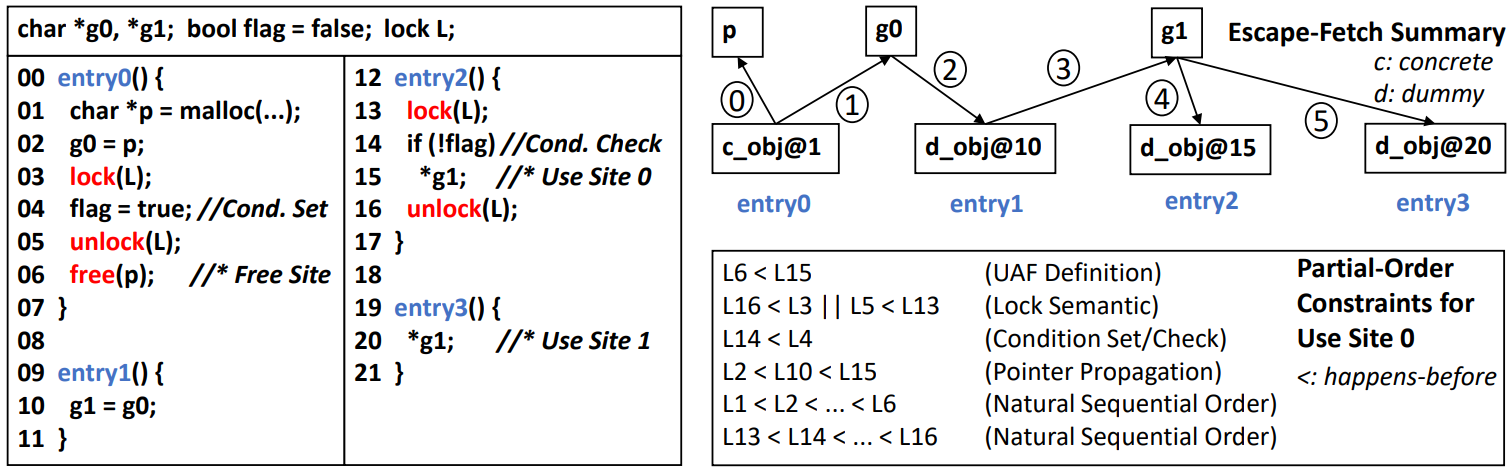
\includegraphics[scale=.4]{images/uafx-example.png}
    \caption{Example of code entry points and how they are handled by UAFX.}
    \label{fig:uafx-example}
\end{figure}

\subsubsection{Escape-Fetch-based Cross-Entry Alias Analysis}
UAFX treats object assignments to pointers as escapes and retrievals (from "unknown" areas) as fetches. UAFX attempts to construct Escape-Fetch Paths (EFPs) to define aliases that track memory allocation, usage, and deallocation from different access points. This is necessary because, from the perspective of a single function, an object may have an unknown origin (as is commonly the case with an externally initialized pointer, such as \texttt{g1} in \texttt{entry3}).

\subsubsection{Systematic Partial-Order Constraint-based UAF Validation}
Once the aliases/paths have been confirmed, UAFX verifies that the conditions for a UAF actually exist.
If, for example, there is a check on a flag (\texttt{entry0}, \texttt{entry2}) that is manipulated by multiple entry functions and used to prevent a UAF on a critical pointer, that path must be discarded.

\subsubsection{Workflow}
We can break down UAFX's workflow as follows:
\begin{enumerate}
    \item \textbf{Identifying entry functions.} This is done semi-automatically, starting with:
    \begin{itemize}
        \item \textit{General call analysis}: functions that serve as entry points typically have no callers in the program, so they are candidates.
        \item \textit{Software-based heuristics}: the paper uses drivers as an example; these typically have entry points in a \texttt{file\_operations} structure, which makes them easy to identify.
    \end{itemize}
    After these initial automated steps, a manual review is conducted to exclude unnecessary candidates or to add others.

    \item \textbf{Code analysis and summary for each entry.} The entry functions are analyzed, and all escape/fetch objects, critical regions, and condition sets/checks (such as the flag in the example) are identified. UAFX generates a summary of all possible paths (in Figure \ref{fig:uafx-example}, the graph in the upper right).

    \item \textbf{Cross-entry detection of free and use sites with aliases.} UAFX considers all sites where memory regions are freed and used as potential candidates for UAF. In the example, with the path \texttt{entry0}-\texttt{entry3}, defined as follows (between the \textit{free} operation on line 6 and the \textit{use} operation on line 20):
    \begin{center}
        (c\_obj@1 $\longrightarrow$ g0 $\longrightarrow$ d\_obj@10 $\longrightarrow$ g1 $\longrightarrow$ d\_obj@20)
    \end{center}
    there is a potential UAF.

    \item \textbf{UAF Validation.} UAFX considers all candidates and evaluates their constraints within the path (order, locks, set/check conditions) to determine whether each one is actually a vulnerability.
    It also verifies that the free and use sites actually access the same object, taking into account the entire escape-fetch path.
    For this purpose, SMT solvers can be used (the paper cites z3 as an example).
\end{enumerate}

\subsubsection{Thread tracking}
Since some UAFs are caused by race conditions, UAFX recognizes two types of thread-related lifecycles:
\begin{itemize}
    \item \textbf{Thread creation}: calls that create child threads (\texttt{pthread\_create}, \texttt{fork}). UAFX retrieves information from these events (e.g., the thread's entry function or parameters)

    \item \textbf{Thread joins} (\texttt{pthread\_join}, \texttt{wait}): events that ensure threads exit before a certain point in the parent thread. UAFX pairs each exit event with its corresponding creation event to track the entire thread lifecycle.
\end{itemize}

\subsubsection{UAFX and CVE-2025-21756}
Speaking specifically about our case, UAFX may not be able to automatically identify the UAF for CVE-2025-21756 because of two main issues.

A first obstacle could be identifying the entry functions. As described earlier, automatic identification of candidates occurs for functions that have no callers, but this is not the case here because the functions that operate on socket objects are instead called by other functions.
This could be resolved in the second step of the identification process, namely by manually adding the functions to the set of candidates.

Another, more significant obstacle is the difficulty explicitly described in tracking reference counts (page 9 of the paper \cite{ndss-uafx}, \textit{Reference Count Mechanisms}).
UAFX intentionally avoids analyzing candidates involving reference counts, which is, in fact, the main cause of CVE-2025-21756, because of the excessive number of false positives that would be generated, in order to maintain high precision (but lower recall).
Despite this, it would be theoretically possible to extend UAFX with the help of other previouslky mentioned tools (here and in UAFX's paper): LinKRID (page 14), CRCount, and FreeWill (page 15) can, with some modifications, be used together with UAFX to increase accuracy on reference count problems.

As described in section
% TODO - riferimento quando c'è capitolo e descrizione là
, we tried making a slight modification to the UAFX code to see if we could also detect the reference counting issue.

\subsection{CountDown}
CountDown is a fuzzer for the Linux kernel, presented at CCS 2024 \cite{countdown} and, unlike UAFX, it's specifically designed to detect memory timing errors caused by incorrect handling of reference counters. Unlike traditional fuzzers, which are primarily driven by code coverage, CountDown uses operations on reference counters as feedback to identify sequences of system calls that could potentially alter the lifecycle of those same objects. The tool is built on top of Syzkaller and extends its strategies for generating and mutating test programs.

During execution, CountDown instruments the kernel to associate increments, decrements, and accesses to reference counters with the system calls that triggered them. Based on this information, it establishes relationships between system calls that operate on the same counters and assigns them a higher probability of being combined in the generated tests. The tool can also repeatedly insert operations that decrement a counter, in an attempt to trigger the object's deallocation, followed by operations that continue to access it. In this way, fuzzing is directed toward sequences that can more effectively expose UAFs caused by incorrect operations on counters.

CountDown's approach is based on the idea of refcount-driven fuzzing to achieve two macro-objectives:
\begin{itemize}
    \item \textit{Identification of refcount-based relationships between syscalls}: instead of relying solely on syscall signatures or coverage, CountDown correlates syscalls that operate on the same object (\textit{shared refcounts}).

    \item \textit{Systematic exposure of UAF bugs}: through targeted mutations, the tool attempts to force an object's refcount to zero and subsequently access that object via syscalls that share its reference.
\end{itemize}

\subsubsection{Workflow}
CountDown's workflow can be broken down into three main phases:
\begin{enumerate}
    \item \textbf{Kernel instrumentation and logging}: CountDown instruments the refcount APIs in the Linux kernel to log every refcount operation using a 4-element tuple:
    \begin{center}
        $<S, O, \delta, V>$
    \end{center}
    where a syscall S updates the refcount O of a refcount by a value $\delta$. V is the final value.

    The instrumented APIs are listed in the following table:

    \begin{center}
        \begin{tabular}{|c|c|}
            \hline
            \textbf{Name} & \textbf{Description} \\\hline
            \texttt{refcount\_set} & set refcount to the given value \\\hline
            \texttt{refcount\_add} & add the given value to refcount \\\hline
            \texttt{refcount\_inc} & increase refcount by 1 \\\hline
            \texttt{refcount\_dec} & decrease refcount by 1 \\\hline
            \texttt{refcount\_add\_not\_zero} & add given value to refcount if refcount is not 0 \\\hline
            \texttt{refcount\_inc\_not\_zero} & increment if the refcount is not 0 \\\hline
            \texttt{refcount\_dec\_not\_one} & decrement if the refcount is not 1 \\\hline
            \texttt{refcount\_dec\_if\_one} & decrement if the refcount is 1 \\\hline
            \texttt{refcount\_dec\_and\_test} & decrement refcount and check if result is 0 \\\hline
            \texttt{refcount\_sub\_and\_test} & subtract value from refcount and check it with 0 \\\hline
        \end{tabular}
        \label{table:refcounts}
    \end{center}
    
    To identify the same object across different virtual machines (VMs), it uses a checksum of the call stack at the time of the object's initialization through \texttt{refcount\_set}.

    CountDown creates a RAI map (\texttt{refcount-address-ID}) to link the addresses of the refcounts with their refcount IDs.\\
    When a refcount is initialized, a new entry in the RAI map is created with its address and ID.\\
    When a refcount reaches zero, the entry is removed from the map.\\
    When a refcount is incremented or decremented, CountDown searches the address in the map to find its ID and records the operation.

    During fuzzing, to connect refcount operations with syscalls, CountDown needs to record the Syzkaller syscall number (NR) for each operation. This is done in a thread-safe manner in order to avoid race condition, since the Linux kernel utilizes multiple threads to execute parallelized syscalls.

    While tracking the refcount values, CountDown considers that one syscall may modify a refcount many times, but it only cares about the final variation ($\delta$). In order to do so, every refcount API listed in table \ref{table:refcounts} is modified to record every single refcount change.
    This data is kept in a two-dimension table (one for the syscall number, one for the refcount ID), in which every entry records the current $\delta$ and the current $V$. 

    \item \textbf{Reworking relationships between system calls}: CountDown constructs multiple relations among syscalls and refcounts starting from the refcount operations mapped in the 4-tuple format $(S, O, \delta, V)$.
    
    First, it identifies syscalls that effectively change the refcount of any object. It remaps a set of 4-tuples in a new map, where the key is the refcount ID and the value is a set of syscalls and their changes to the refcount ($\delta$), avoiding relations between syscalls from different programs (which can quickly become unrealiable).
    
    Based on the shared refcounts, every relation is reworked in a new one defined as \texttt{RefcntRelation}. The assumption is that, if two syscalls access the same refcount within one execution, they have a stronger relation with respect to triggering more complicated refcount operations. Each syscall set associated with a specific refcount is then split into a set of syscalls pairs. Following that, CountDown creates the syscall relation table, where each unique pair of syscalls has an entry and the value is the number of shared refcounts accessed by both.

    \begin{center}
        \begin{figure}[h]
            \centering
            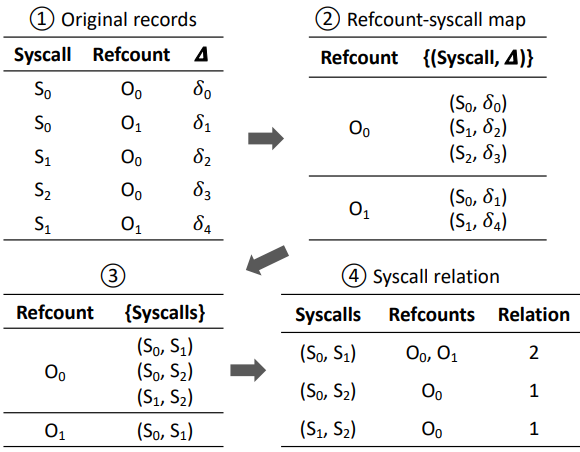
\includegraphics[width=0.7\linewidth]{images/countdown-step2.png}
            \caption{Example of refcount-based syscall relation construction.}
            \label{fig:countdown-step2}
        \end{figure}
    \end{center}
    
    As explained in the paper, this newly constructed relation is more efficient in detecting refcount-related UAF bugs. However, the kernel code base is very large and refcount operations are not densely distributed. To solve the problem, the \texttt{RefCntRelation} is merged with the Syzkaller's standard \texttt{SyzRelation} and handled based on the fuzzing time. At the beginning of fuzzing, CountDown assigns a high priority to the original coverage-based relation to quickly explore more kernel code. As time goes on, it allocates more weight to CountDown's own relation so that the fuzzer can focus on testing complex refcount operations. This can be represented as the following formula:

    \begin{center}
        $OverallRelation = log_2(SyzRelation) + k * log_2 (RefcntRelation)$
    \end{center}

    $k$ starts with a small value and is incremented every time after testing a fixed number of test cases.

    Since fuzzers are non-deterministic, different kernel instances can gather different relations. When a new one is received from one VM, CountDown synchronizes it across all instances (to ensure that the other instances can directly make use of it) by fetching each VM's report, merging them and then distributing the result to all instances.

    \item \textbf{Guided program mutation}: CountDown uses the learned relationships to generate new programs. It starts by using the mutators from previous fuzzing tools (like Syzkaller) to mutate the program. Having assigned higher weights to refcount-based relations, the mutation will prefer combining syscalls that are strongly related regarding refcount operations.  

    Then it creates a new mutator that combines refcount-related syscalls more aggressively. CountDown chooses one target program and runs it in order to collect all accessed refcounts. It will update the refcount-syscall map if the execution triggers new records. To mutate the program, it will randomly select a refcount from the collected set. If a refcount was accessed multiple times, it will have a higher probability to be selected. 

    CountDown then searches the map for syscalls that operate on this refcount and selects one for insertion into the program, which is done reusing Syzkaller's logic, preferring a later position, because the syscalls at the beginning may work on the initialization of resources and refcounts.

    In addition to new code coverage, CountDown considers any program that exhibits a new \texttt{(syscall, refcount)} pair never seen before to be "interesting" and saves it for future changes. This is done while fuzzing through checking whether the execution triggers new code coverage or a new refcount operation, which was previously missed. If that's the case, it saves the new program into the input queue for further mutations and updates the refcount-syscall map with the new entry.

    As a final but important point, a triggered refcount error will not immediately result in a memory error. CountDown needs to trigger more operations to make the kernel release the object and access it through dangling references. It does so by inserting more refcount-related syscalls into the executed program in order to reduce the gap between a refcount bug and a UAF, so that sanitizers like KASAN can capture it.
\end{enumerate}

\subsubsection{Limitations}
Although CountDown is optimized to detect UAFs with refcounts, it still has some limitations:
\begin{itemize}
    \item \textbf{Generic refcounts}: some refcounts (such as those in the AppArmor security module) are used by nearly all syscalls, creating "noise" and artificial relationships that CountDown must filter out to maintain accuracy.

    \item \textbf{Coverage trade-off}: because it focuses heavily on refcount logic, CountDown may record slightly lower total code coverage (approximately 1.8\% – 4.3\% less) than Syzkaller, as it ignores paths unrelated to object management.

    \item \textbf{Instrumentation overhead}: although optimized through selective logging (excluding interrupts and asynchronous tasks), the constant monitoring of every refcount operation introduces a higher computational load than traditional fuzzing.
\end{itemize}

\chapter{CVE-2025-21756}

\section{Overview}
CVE-2025-21756 is a use-after-free vulnerability identified in the Linux kernel's AF\_VSOCK subsystem, which is used for communication between hosts and virtual machines. The vulnerability allows a local attacker to gain elevated privileges (up to root) by exploiting incorrect management of the socket object lifecycle within the kernel.

The problem arises during specific sequences of operations on vsock sockets, leading to the dereferencing of memory structures that have already been freed and, consequently, to kernel memory corruption. Specifically, an attacker could exploit this vulnerability to achieve privilege escalation.

\section{The VSOCK subsystem}\label{vsock_subsystem}
VSOCK is a component of the Linux kernel that manages communication between a virtual machine (\textit{guest}) and the system hosting it (\textit{host}). It was developed in response to the need to provide a method of communication between the two entities that offers better performance than traditional network interfaces. Unlike TCP/IP sockets, which are based on IP addresses and network protocols, vsock sockets use an addressing model specific to virtualised environments. Communication via vsock utilises a pair of identifiers:
\begin{itemize}
    \item \textbf{CID (Context IDentifier)}: uniquely identifies an endpoint (host or VM)
    \item \textbf{Port}: similar to TCP/UDP ports
\end{itemize}
Some relevant CID values may include:
\begin{itemize}
    \item \texttt{VMADDR\_CID\_HOST}: represents the host
    \item \texttt{VMADDR\_CID\_LOCAL}: local communication
    \item specific CIDs assigned to individual VMs
\end{itemize}
The advantage of this model is that it avoids the overhead associated with the IP stack.\\
Communication takes place via two transport networks:
\begin{itemize}
    \item \textbf{G2H (guest-to-host)}: these are executed on the guest and are usually device drivers. We distinguish between three types:
    \begin{itemize}
        \item \textit{virtio-transport}: typical of KVM/QEMU, it uses virtqueues located within the guest as buffers, but the host also reads from and writes to them.

        \item \textit{vmci-transport}: VMWare's proprietary for H2G/G2H.

        \item \textit{hyperv-transport}: based on Hyper-V VMBus, designed specifically for Microsoft environments.
    \end{itemize}

    \item \textbf{H2G (host-to-guest)}: these are run on the host and usually provide device emulation for the guest. There are two types:
    \begin{itemize}
        \item \textit{vhost-transport}: host-side backend for virtio-transport.

        \item \textit{vmci-transport}: VMWare's proprietary for H2G/G2H.
    \end{itemize}
\end{itemize}
To illustrate communication between the host and the guest, we can use QEMU, an open-source emulator and virtualisation program, as an example. When creating a virtual machine, the structure will be as follows:
\begin{itemize}
    \item \textit{virtio-transport} on the guest
    \item \textit{vhost-transport} on the host: provides in-kernel device emulation to the guest and uses \texttt{ioeventfd} and \texttt{irqfd} to receive and send events to the guest.
\end{itemize}
\begin{figure}[h]
    \centering
    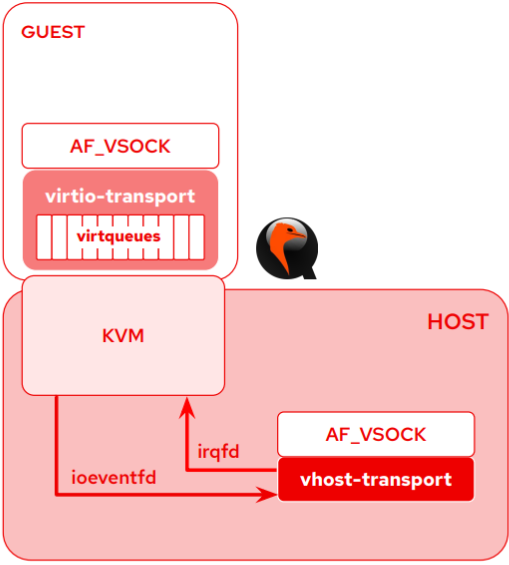
\includegraphics[scale=.4]{images/vsock.png}
    \caption{Example of a VSOCK communication structure.}
    \label{fig:vsock}
\end{figure}
Both provide an interface to the socket layer via the vsock core and exchange packets with virtio queues (\textit{virtqueues}).\\
KVM (Kernel-based Virtual Machine) turns the host OS into the VM's hypervisor, enabling it to manage the CPU and memory directly.

\subsubsection{Virtqueues}
These are shared buffer queues in memory that allow the two parties to communicate bidirectionally (even though a single virtqueue is dedicated to a single direction) while maintaining low overhead.\\
In \textbf{split virtqueue} mode (classic), they are based on three main shared memory areas:
\begin{itemize}
    \item \textbf{Descriptor Area}: contains the buffer metadata (the guest's physical address and length).

    \item \textbf{Available Ring}: a list of buffers that the driver has added and which are ready to be consumed by the host device.

    \item \textbf{Used Ring}: a list of buffers that the device has finished processing and is returning to the driver.
\end{itemize}
The \textbf{packed virtqueue} mode, on the other hand, uses a more modern and compact layout, merging the available and used rings, thereby improving the performance of the processor cache.\\
The operation can be broken down into the following stages:
\begin{enumerate}
    \item \textbf{Insertion}: the VirtIO (guest) driver places the buffers in the \textit{descriptor area} and updates the \textit{available ring}.

    \item \textbf{Notification (Kick)}: The driver sends a notification to the device ("doorbell") to indicate that new data is available.

    \item \textbf{Processing} of data by the host.

    \item \textbf{Completion}: the host updates the \textit{used ring} and sends an interrupt to the guest to signal completion.
\end{enumerate}
The virtqueue backend (which actually manages the queue on the host) can be \textbf{QEMU}, with full emulation, as in the case under consideration, or \textbf{vhost}: the backend runs within the host kernel (vhost-net/vhost-blk), allowing the driver to communicate directly with the kernel without going through QEMU's user space, thereby drastically reducing latency.

\subsubsection{Internal architecture of VSOCK}
From an implementation perspective, each vsock socket is represented in the kernel by a data structure (\texttt{struct vsock\_sock}), which extends the generic socket structures (\texttt{struct sock}). These objects are managed via:
\begin{itemize}
    \item \textbf{status lists}:
    \begin{itemize}
        \item \textit{bound sockets}: associated with a port;
        \item \textit{unbound sockets}: created but not yet associated;
    \end{itemize}
    \item \textbf{connection queue}: handling of incoming requests;
    \item \textbf{reference counting}: a fundamental mechanism for managing the life cycle of objects.
\end{itemize}
When consistency in the management of these elements is lacking, there is a risk of encountering the problems mentioned above, exposing the system to risks and attacks.

\subsubsection{The life cycle of a VSOCK socket}
Typically, a vsock socket goes through the following stages:
\begin{enumerate}
    \item \textbf{Creation} (\texttt{socket()}): memory is allocated for the data structure, which is then added to the \textit{unbound} list.

    \item \textbf{Binding} (\texttt{bind()} or autobind): the socket is associated with a port and is consequently added to the \textit{bound} list.

    \item \textbf{Connection} (\texttt{connect()} / \texttt{accept()}): the actual communication channel is established.

    \item \textbf{Release} (\texttt{close()}): when the socket is no longer needed, it is removed from the internal structures, its reference count is decremented and, if this reaches zero, its memory is deallocated.
\end{enumerate}

\section{Cause of the vulnerability}
The cause of CVE-2025-21756 may be considered trivial at the code level, but given that certain preconditions are required for the problem to occur, and given that the result is not readily apparent, identifying it was by no means straightforward.

% TODO - dettagli

\section{Test case presented by the developers}
Let's start with a test case provided by the maintainers of the VSOCK module for the Linux kernel, who, after releasing the patch, made it available to allow users to check whether their system is affected by the issue.
\clearpage
\begin{figure}[h]
    \centering
    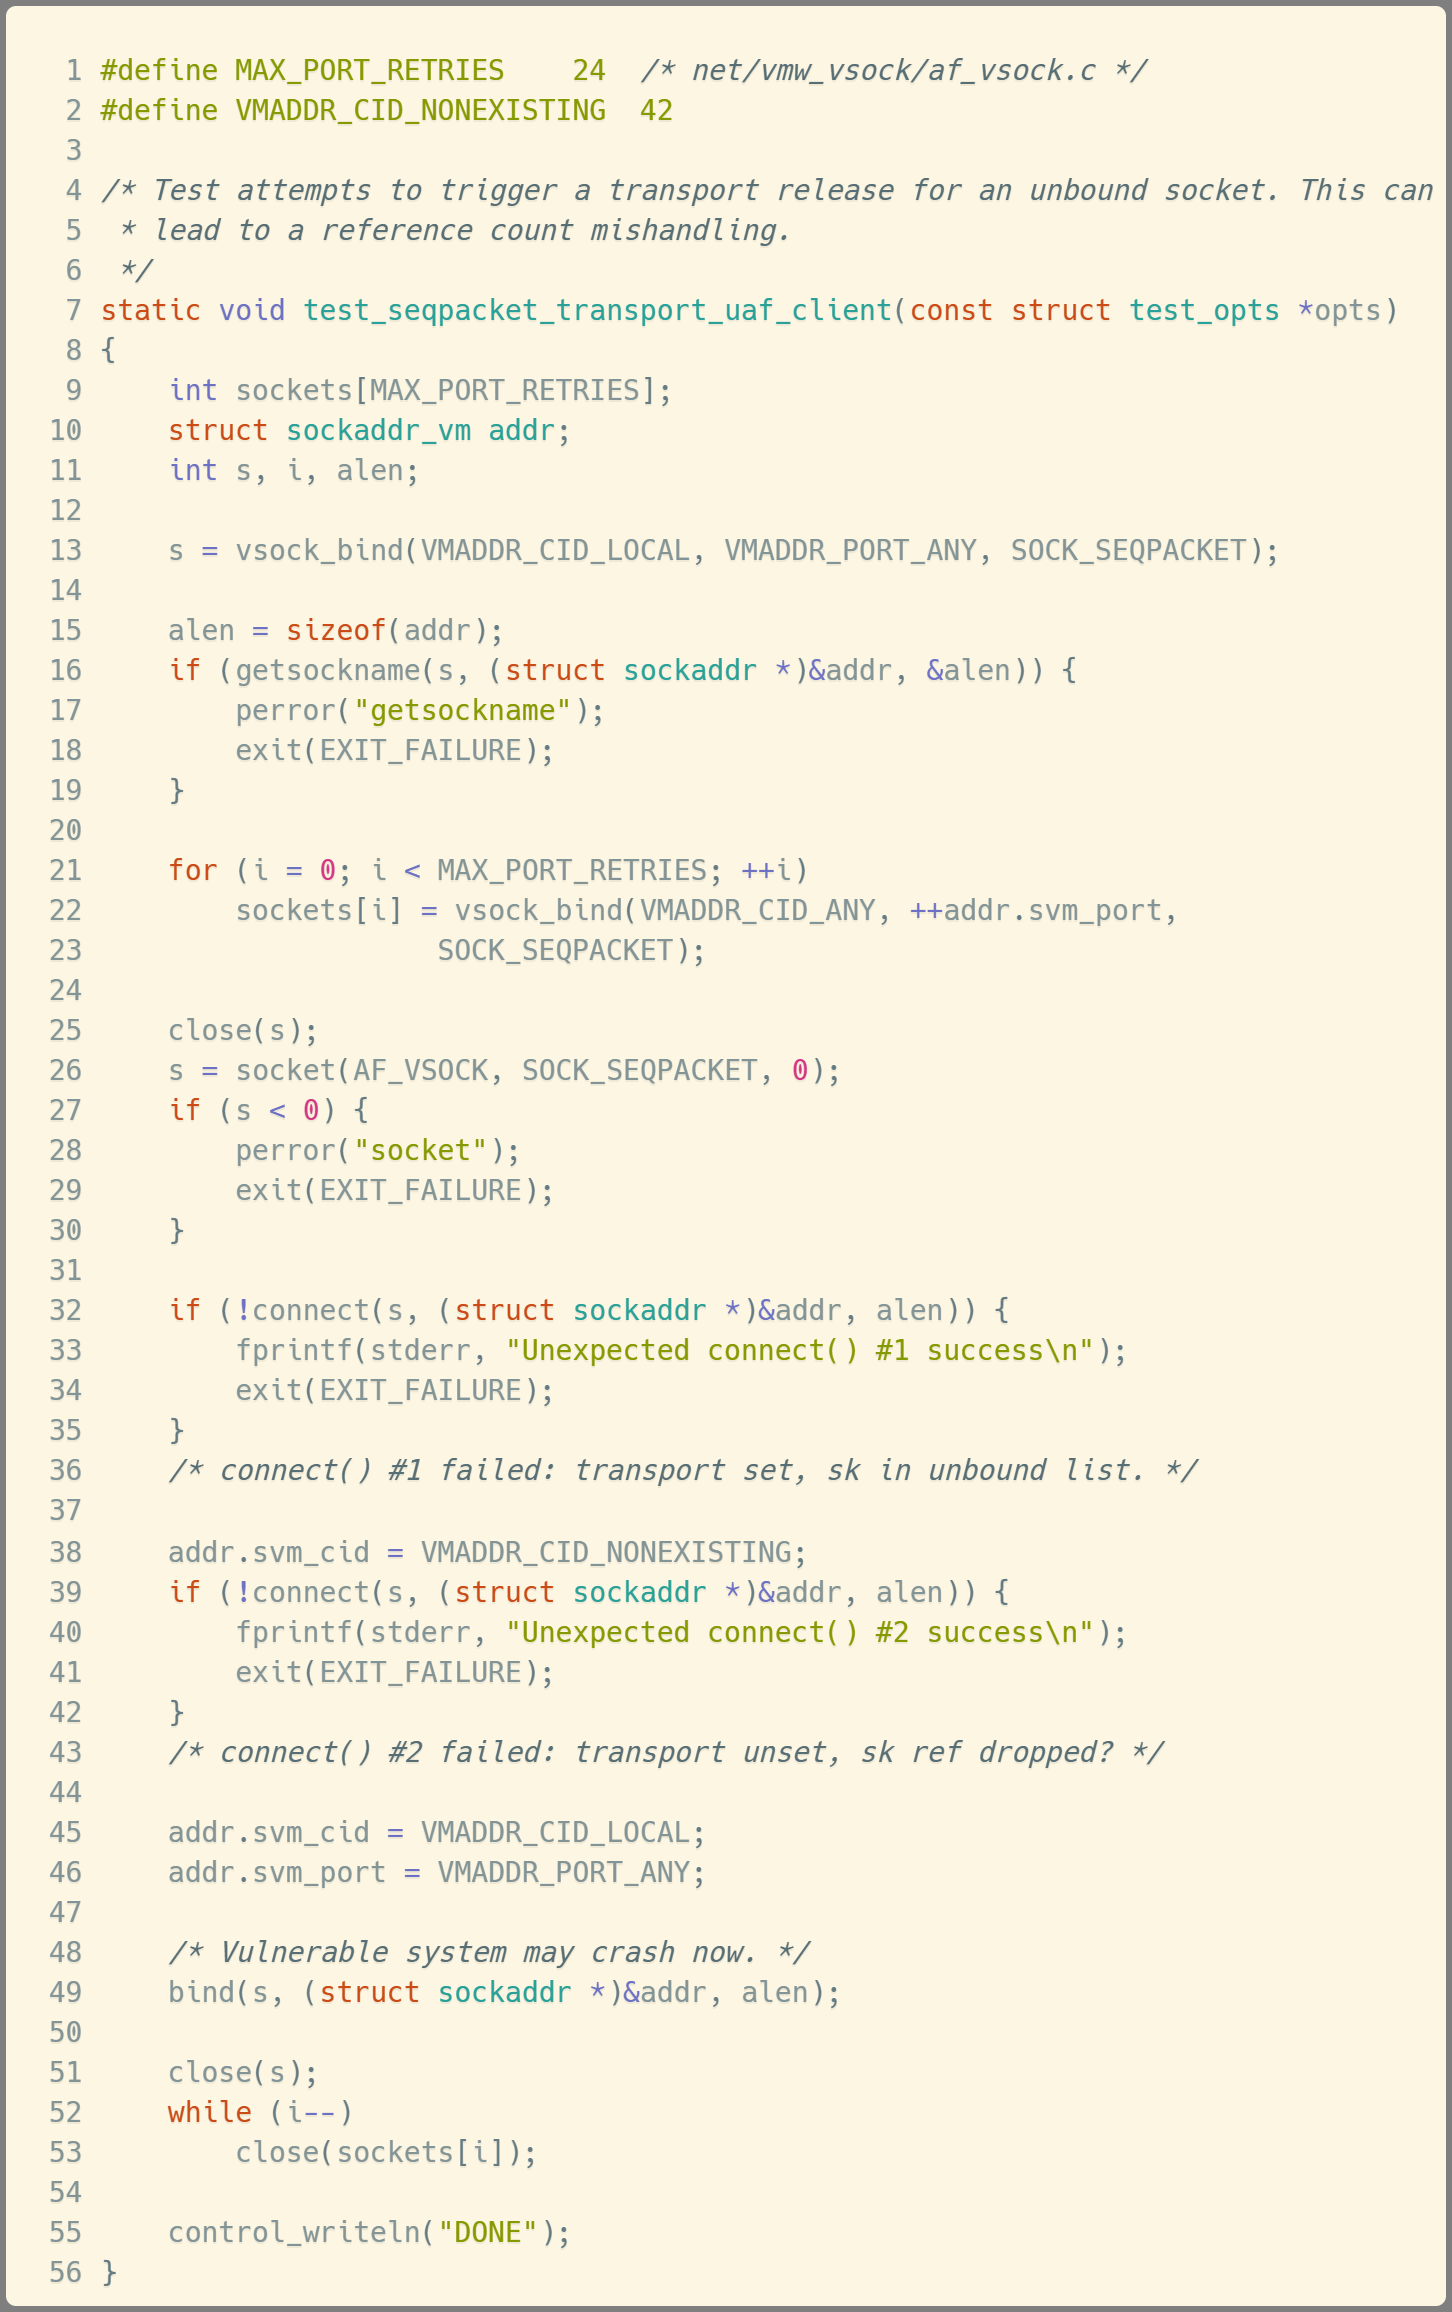
\includegraphics[scale=.2]{images/test_case.png}
    \caption{The test case provided by the maintenance developers.}
    \label{fig:test_case}
\end{figure}
\noindent The test case in question does not lead to a privilege escalation, but causes the kernel to crash on vulnerable systems. By examining it step by step, it is possible to understand what is going wrong in the reference counting mechanism associated with a vsock socket.

\section{Functions involved}

\section{Patches and mitigation measures}

\section{Overview of the exploit}


\chapter{Use-after-free vulnerabilities that exploit reference count errors}

\chapter{Static analysis tools}

\chapter{Application of <tool>}

%
%			BIBLIOGRAFIA
%
\begin{thebibliography}{00}

\bibitem{fosspost}
Linux Market Share Statistics 2026: Desktop, Server and Enterprise Adoption Trends
\url{https://fosspost.org/linux-market-share-statistics/}, 2026.

\bibitem{ndss-uafx}
Statically Discover Cross-Entry Use-After-Free
Vulnerabilities in the Linux Kernel \url{https://www.ndss-symposium.org/wp-content/uploads/2025-559-paper.pdf}, 2025

\bibitem{countdown}
CountDown: Refcount-guided Fuzzing for Exposing Temporal Memory Errors in Linux Kernel \url{https://dl.acm.org/doi/epdf/10.1145/3658644.3690320}, 2024

\end{thebibliography}

\end{document}